\chapter{Introduction}\label{chapter:introduction}
The simulation of fluids is part of our daily life, even if many do not have this in mind. It facilitates the planning phase of vehicles, airplanes and boats by allowing the aerodynamic properties to be determined even before the first prototype has been built \parencite{tsubokura2009computational}. A weather forecast as precise as we know it today would not be possible if we could not simulate the air flows of the earth \parencite{kimura2002numerical}. And the simulation of fluids also plays a role in medicine, for example, to better understand blood flow in the human heart \parencite{peskin1977numerical}. Many designers and artists are working to deliver the greatest possible immersion to the viewer in games and films \parencite{gilland2009elemental}. Compared to the design for instance of 3D objects, it is very complex and time-consuming to create realistic looking artificial waves with all the splashes and foam \parencite{gilland2009elemental}.
\par Existing solutions are often very computationally intensive and lead to compromises between speed and accuracy, resolution or size and thus to the believability of the simulation. Especially in games you only have a few milliseconds until the result has to be delivered. Only the immense parallel computing power of graphics cards made it possible to compute dense fluids in real time. 
\par Deep Learning has become state-of-the-art in many areas such as object recognition in recent years \parencite{lecun2015deep}. Deep neural networks also appear to be capable of realistically mimicking physical phenomena with the advantage of doing so in a fraction of the time required by conventional solutions \parencite{tompson2017accelerating} \parencite{thuerey2018well}.
\section{$\Phi_\textit{Flow}$ }
$\Phi_\textit{Flow}$ is a toolkit written in Python and currently under development at the TUM Chair of Computer Graphics and Visualization for solving and visualizing n-dimensional fluid simulations. It focuses on keeping every simulation step differentiable which makes it suitable for backpropagation. Backpropagation is required to calculate the gradient of the loss function of Neural Networks to adjust the weights of the network. Being developed on top of TensorFlow, it is not only capable of running on CPUs, but also completely on GPUs. TensorFlow simplifies the implementation of Machine Learning algorithms including the use of Neural Networks for predictions and classification. This makes $\Phi_\textit{Flow}$ a powerful tool to train Neural Networks on fluid simulations and also visualize them by its interactive GUI running in the browser. 
\section{Description of the problem}
This work proposes an implementation to solve the pressure equation - the most computationally intensive part of Eulerian fluid simulations. Being as efficient as possible is crucial for fast simulations and thus most importantly for the training of neural networks. $\Phi_\textit{Flow}$ already comes with its own pressure solver running directly in TensorFlow. However, TensorFlows dataflow graph is unnecessarily complex which brings overhead to the computation.
\par TensorFlow offers the possibility to write custom operations ("Custom ops") in C++ to tackle this issue: Writing efficient code to solve a specific problem within the dataflow graph. Furthermore, the CUDA API by Nvidia makes it possible to write low-level CUDA code that runs natively on GPUs. Combining Custom Ops and CUDA kernels lead to a solution that is both efficient and transparent and also compliant to TensorFlow's Tensors which is required within $\Phi_\textit{Flow}$. It can then be compared to the built-in solution of $\Phi_\textit{Flow}$.
\section{Outline}
Chapter 2 discusses past research in this area.\\
Chapter 3 repeats the theoretical and mathematical background necessary for this work.\\
In Chapter 4 I present how I improved the Pressure Solve on GPUs.\\
In chapter 5 I show the results and compare them with those from $\Phi_\textit{Flow}$.\\
Chapter 6 summarizes and gives suggestions for further work.\\

\begin{figure*}[t]
    \centering
	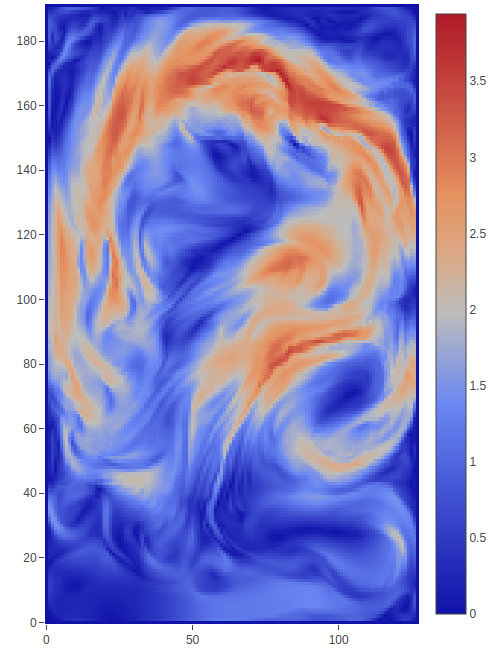
\includegraphics[scale=0.85]{figures/phiflow}

	\caption{Grid-based fluid simulation in $\Phi_{flow}$}
\end{figure*}